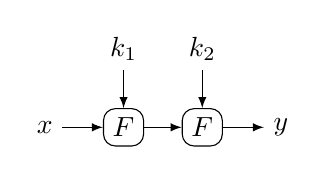
\begin{tikzpicture}
\node (x)  {$x$};
\node (f1) [right of=x, rounded corners=1ex, draw] {$F$};
\node (f2) [right of=f1, rounded corners=1ex, draw] {$F$};
\node (y)  [right of=f2] {$y$};
\node (k1) [above of=f1] {$k_1$};
\node (k2) [above of=f2] {$k_2$};
\draw [-latex] (x) -- (f1);
\draw [-latex] (f1) -- (f2);
\draw [-latex] (f2) -- (y);
\draw [-latex] (k1) -- (f1);
\draw [-latex] (k2) -- (f2);
\end{tikzpicture}